\chapter{Experimentación y Resultados}
\label{chapter:experimentacion_resultados}

\section{Conjuntos de datos}

Para comenzar la experimentación vamos a hacer un repaso de los conjuntos de datos y la técnica seguida para realizar la misma. En primer lugar cabe decir que al ser un problema no supervisado en origen no tendríamos forma de saber nuestro acierto en el problema. En este tipo de casos hay dos aproximaciones: estimar el acierto o utilizar conjuntos que sí están clasificados y obtener de esta forma el acierto. La segunda de las alternativas es la que vamos a seguir en este estudio y es la que se suele denominar como problema semisupervisado. 

Para tomar este camino necesitamos conjuntos en los que tengamos disponible la clasificación de datos anómalos y no anómalos. Estos conjuntos de datos han sido tomados de la web Otlier Dection Datasets \cite{shebuti_ryana_odds_2016}, librería mantenida por la universidad Stony Brooks.

Estos conjuntos de datos están en formato Matlab, formato que puede ser fácilmente leído por la librería SciPy. Estos conjuntos de datos vienen con información de cabecera, versión e incluso algunos con una breve descripción o resumen si dispusieran de ella. Lo importante es que los datos vienen divididos en dos, primero un vector que contiene una lista con los vectores que componen los datos y en segundo lugar un vector con las etiquetas donde $0$ significa que el dato no es anómalo y $1$ que sí lo es.

\begin{figure}[H]
	\centering
	\label{dataset_matlab}
	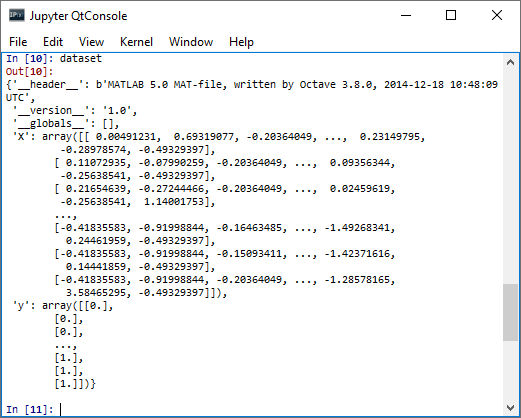
\includegraphics[scale=0.8]{imagenes/datasets_matlab}
	\caption{Contenido de los conjuntos de datos}
\end{figure}

Como podemos ver ``X'' contiene el conjunto de datos y el campo ``y'' contiene las etiquetas para los mismos.

En algunos de estos conjuntos de datos podemos encontrar lo que conocemos como valores perdidos o en inglés ``missing values''. Estos valores vienen reflejados con ``NAN'' en los conjuntos. Estos valores no sólo no nos son de interés si no que además nuestros modelos no están preparados para poder trabajar con ellos por lo que tenemos que decidir que transformación aplicamos para poder emplear los conjuntos de datos. La decisión tomada para estos valores ha sido la de eliminar las instancias que presenten valores perdidos. Esta decisión se basa en que, si estas instancias son anómalas no tenemos forma alguna de tratar con ellas porque no disponen de valores numéricos en sus campos y por tanto nuestros modelos no son aptos para resolver el conflicto. Esto no excluye el hecho de que estas instancias puedan ser anomalías reales. Por ejemplo pensemos en un sistema de frenos que sufre una rotura de alguno de sus sistemas. Si estos sistemas poseen sensores que recopilan datos es muy probable que estos sensores no tomen valores y por tanto dispongamos de valores perdidos precisamente porque la instancia es anómala. Esto se discutirá un poco más en profundidad cuando hablemos del trabajo futuro, de momento la decisión ha sido suprimir estas instancias.

Dentro de todos los conjuntos de datos que contiene la librería nosostros vamos a utilizar los siguientes:

\begin{table}[H]
	\begin{tabular}{|l|l|l|}
		\hline
		\multicolumn{1}{|c|}{{\ul \textbf{Nombre}}} & \multicolumn{1}{c|}{{\ul \textbf{Dimensionalidad}}} & \multicolumn{1}{c|}{{\ul \textbf{Número de instancias}}} \\ \hline
		annthyroid                                  & 6                                                   & 7200                                                     \\ \hline
		arrhythmia                                  & 274                                                 & 452                                                      \\ \hline
		breastw                                     & 9                                                   & 683                                                      \\ \hline
		cardio                                      & 21                                                  & 1831                                                     \\ \hline
		glass                                       & 9                                                   & 214                                                      \\ \hline
		ionosphere                                  & 33                                                  & 351                                                      \\ \hline
		letter                                      & 32                                                  & 1600                                                     \\ \hline
		lympho                                      & 18                                                  & 148                                                      \\ \hline
		mammography                                 & 6                                                   & 11183                                                    \\ \hline
		mnist                                       & 100                                                 & 7603                                                     \\ \hline
		musk                                        & 166                                                 & 3062                                                     \\ \hline
		optdigits                                   & 64                                                  & 5216                                                     \\ \hline
		pendigits                                   & 16                                                  & 6870                                                     \\ \hline
		pima                                        & 8                                                   & 768                                                      \\ \hline
		satellite                                   & 36                                                  & 6435                                                     \\ \hline
		satimage-2                                  & 36                                                  & 5803                                                     \\ \hline
		speech                                      & 400                                                 & 3686                                                     \\ \hline
		thyroid                                     & 6                                                   & 3772                                                     \\ \hline
		vertebral                                   & 6                                                   & 240                                                      \\ \hline
		vowels                                      & 12                                                  & 1456                                                     \\ \hline
		wbc                                         & 30                                                  & 378                                                      \\ \hline
		wine                                        & 13                                                  & 129                                                      \\ \hline
	\end{tabular}
\end{table}

Como podemos ver hay algunos conjuntos con un tamaño razonablemente grande tanto en dimensionalidad como en número de instancias. Esto será discutido modelo por modelo pues los algoritmos basados en subespacios tienen una complejidad dependiente del factorial de la dimensionalidad, es decir, a partir de una cierta dimensionalidad el tiempo que consumen estos algoritmos es demasiado alto.

\section{Experimentación}

Sobre estos conjuntos de datos hemos ejecutado nuestros cinco modelos implementados: HICS, OUTRES, Mahalanobis Kernel, Trinity y LODA. Sobre estas ejecuciones se ha recopilado el porcentaje de acierto sobre ellos, el tiempo consumido en la ejecución y las propias puntuaciones dadas sobre estos conjuntos de datos por los modelos.

Para poder hacer la comparativa con los datos de nuestros modelos he tomado modelos clásicos. Estos modelos se han cogido de la librería PyOD \cite{zhao_pyod:_2019}. De esta librería se han tomado 10 modelos: Angle-Based Outlier Detection (ABOD), Connectivity-Based Outlier Factor (COF), Histogram-Based Outlier Score (HBOS), K Nearest Neighbors (KNN), Local Outlier Factor (LOF), Minimum Covariance Determinant (MCD), One-Class Support Vector Machines (OCSVM), Principal Component Analysis (PCA), Subspace Outlier Detection (SOD) y Stochastic Outlier Selection (SOS). Sobre estos modelos se ha recopilado exactamente la misma información que sobre los nuestros, es decir, el acierto, el tiempo consumido y las puntuaciones de las instancias.

En cuanto a OUTRES podemos estudiar cuándo un subespacio es importante para una instancia completa. Por tanto hemos lanzado otro experimento para intentar analizar los subespacios que son más relevantes para una determinada instancia.

\section{Resultados}

En primer lugar vamos a ver los resultados que obtenemos de todos los modelos sobre todos los conjuntos de datos. Se muestra un gráfico de barras por cada conjunto de datos con el desempeño de cada modelo. Cabe decir que tanto OUTRES como HICS son algoritmos como hemos comentado con una eficiencia muy mala en tiempo. Al ser su complejidad en tiempo dependiente del factorial de la dimensionalidad sólo hemos ejecutado el algoritmo en conjuntos de datos de baja dimensionalidad para poder completar dicha ejecución en un tiempo razonable, aunque como veremos hay algunos conjuntos de datos cuya ejecución ha llevado varias horas.

Veamos primero todos los gráficos con los resultados para poder analizarlos y particularizar posteriormente.

\begin{figure}[H]
	\centering
	\label{annthyroid_accuracy}
	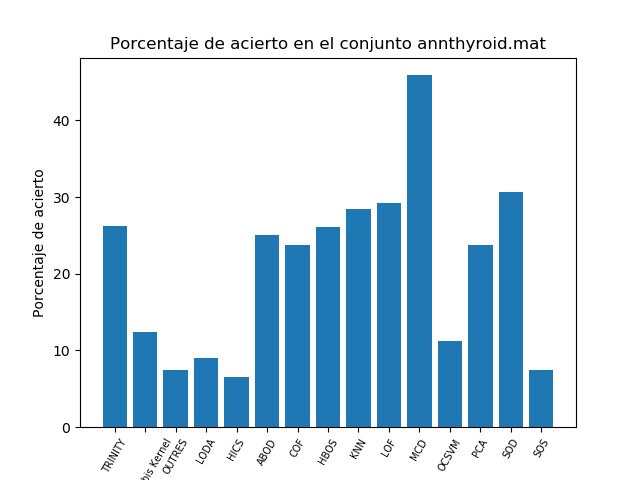
\includegraphics[scale=0.7]{imagenes/imgs-exp1/accuracy/annthyroid}
	\caption{Porcentaje de acierto sobre el conjunto de datos annthyroid}
\end{figure}

\begin{figure}[H]
	\centering
	\label{arrhythmia_accuracy}
	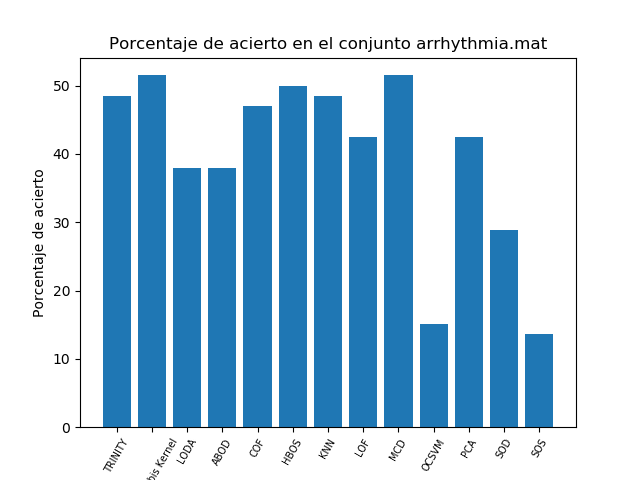
\includegraphics[scale=0.7]{imagenes/imgs-exp1/accuracy/arrhythmia}
	\caption{Porcentaje de acierto sobre el conjunto de datos arrhythmia}
\end{figure}

\begin{figure}[H]
	\centering
	\label{breastw_accuracy}
	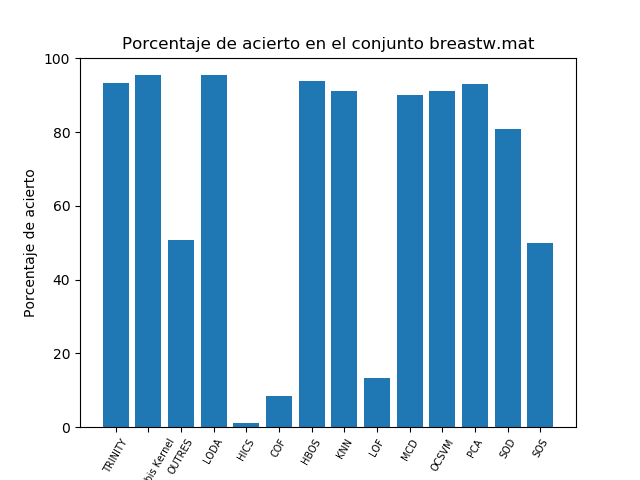
\includegraphics[scale=0.7]{imagenes/imgs-exp1/accuracy/breastw}
	\caption{Porcentaje de acierto sobre el conjunto de datos breastw}
\end{figure}

\begin{figure}[H]
	\centering
	\label{cardio_accuracy}
	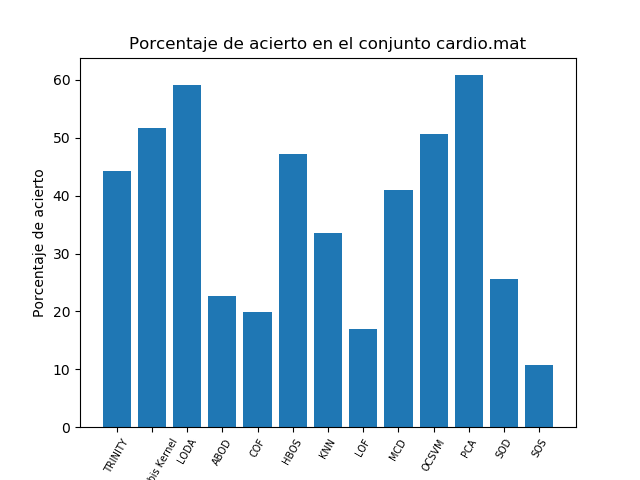
\includegraphics[scale=0.7]{imagenes/imgs-exp1/accuracy/cardio}
	\caption{Porcentaje de acierto sobre el conjunto de datos cardio}
\end{figure}

\begin{figure}[H]
	\centering
	\label{glass_accuracy}
	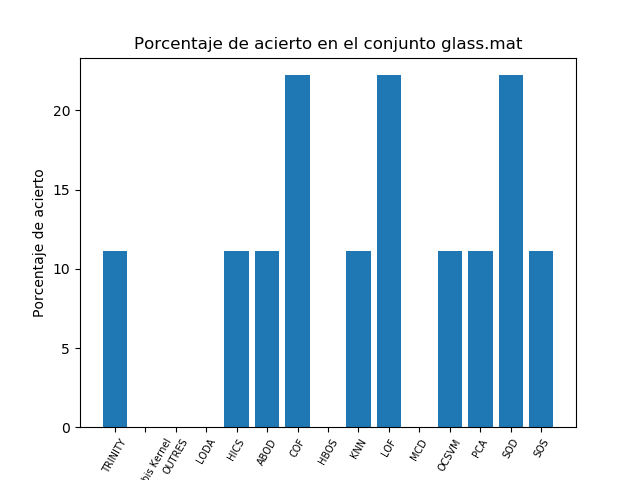
\includegraphics[scale=0.7]{imagenes/imgs-exp1/accuracy/glass}
	\caption{Porcentaje de acierto sobre el conjunto de datos glass}
\end{figure}

\begin{figure}[H]
	\centering
	\label{ionosphere_accuracy}
	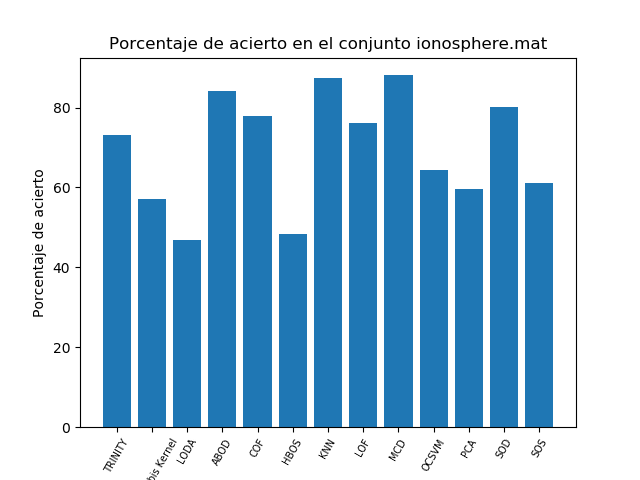
\includegraphics[scale=0.7]{imagenes/imgs-exp1/accuracy/ionosphere}
	\caption{Porcentaje de acierto sobre el conjunto de datos ionosphere}
\end{figure}

\begin{figure}[H]
	\centering
	\label{letter_accuracy}
	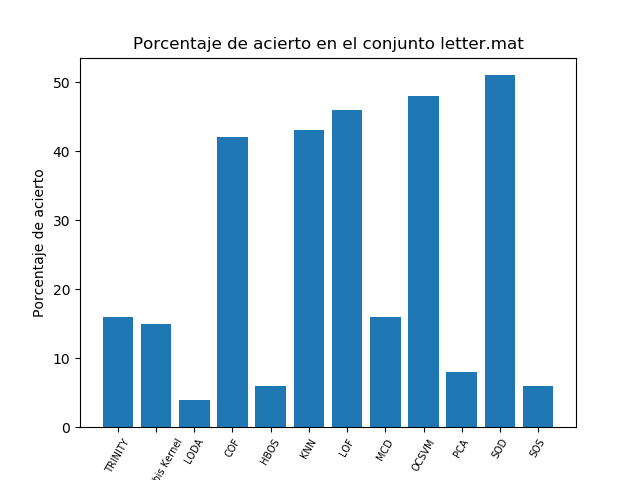
\includegraphics[scale=0.7]{imagenes/imgs-exp1/accuracy/letter}
	\caption{Porcentaje de acierto sobre el conjunto de datos letter}
\end{figure}

\begin{figure}[H]
	\centering
	\label{lympho_accuracy}
	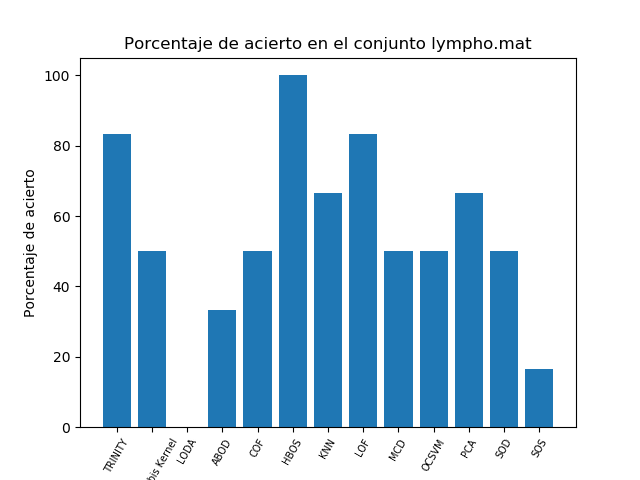
\includegraphics[scale=0.7]{imagenes/imgs-exp1/accuracy/lympho}
	\caption{Porcentaje de acierto sobre el conjunto de datos lympho}
\end{figure}

\begin{figure}[H]
	\centering
	\label{mammography_accuracy}
	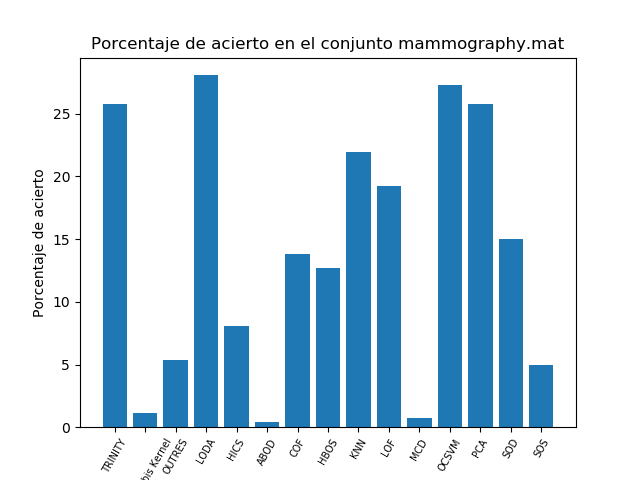
\includegraphics[scale=0.7]{imagenes/imgs-exp1/accuracy/mammography}
	\caption{Porcentaje de acierto sobre el conjunto de datos mammography}
\end{figure}

\begin{figure}[H]
	\centering
	\label{mnist_accuracy}
	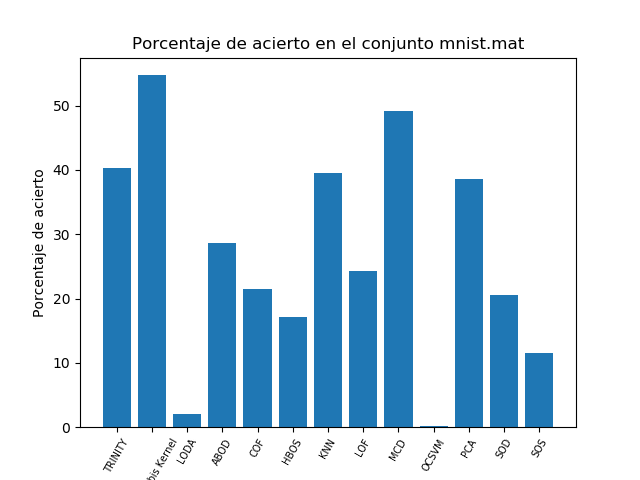
\includegraphics[scale=0.7]{imagenes/imgs-exp1/accuracy/mnist}
	\caption{Porcentaje de acierto sobre el conjunto de datos mnist}
\end{figure}

\begin{figure}[H]
	\centering
	\label{musk_accuracy}
	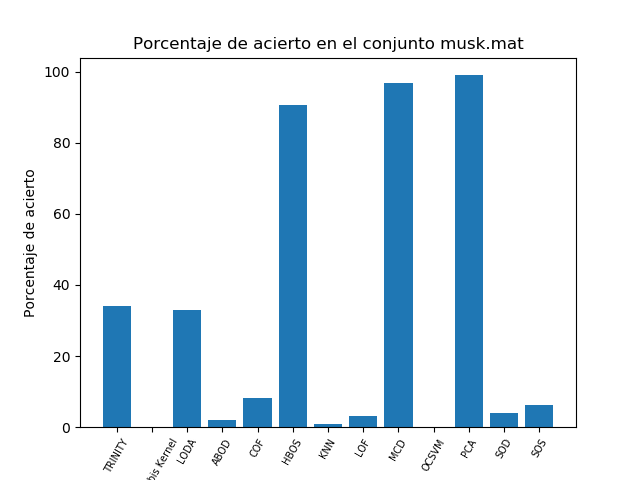
\includegraphics[scale=0.7]{imagenes/imgs-exp1/accuracy/musk}
	\caption{Porcentaje de acierto sobre el conjunto de datos musk}
\end{figure}

\begin{figure}[H]
	\centering
	\label{optdigits_accuracy}
	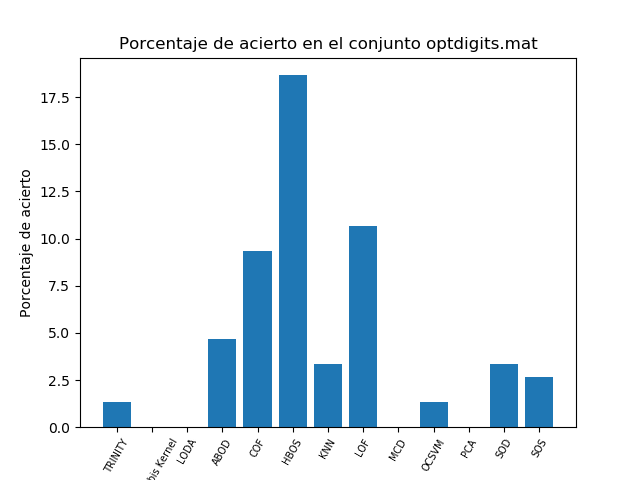
\includegraphics[scale=0.7]{imagenes/imgs-exp1/accuracy/optdigits}
	\caption{Porcentaje de acierto sobre el conjunto de datos optdigits}
\end{figure}

\begin{figure}[H]
	\centering
	\label{pendigits_accuracy}
	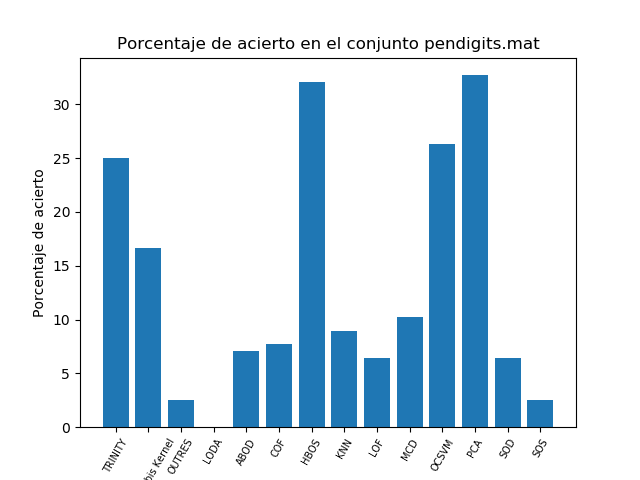
\includegraphics[scale=0.7]{imagenes/imgs-exp1/accuracy/pendigits}
	\caption{Porcentaje de acierto sobre el conjunto de datos pendigits}
\end{figure}

\begin{figure}[H]
	\centering
	\label{pima_accuracy}
	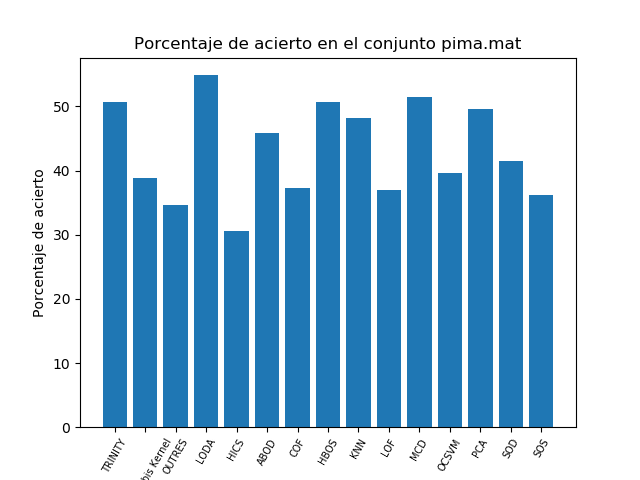
\includegraphics[scale=0.7]{imagenes/imgs-exp1/accuracy/pima}
	\caption{Porcentaje de acierto sobre el conjunto de datos pima}
\end{figure}

\begin{figure}[H]
	\centering
	\label{satellite_accuracy}
	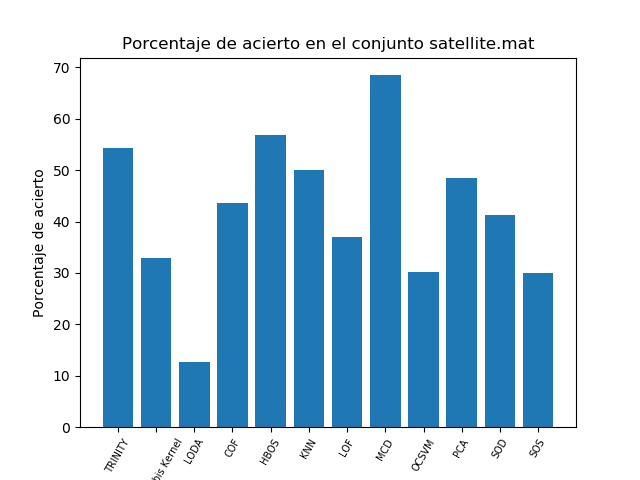
\includegraphics[scale=0.7]{imagenes/imgs-exp1/accuracy/satellite}
	\caption{Porcentaje de acierto sobre el conjunto de datos satellite}
\end{figure}

\begin{figure}[H]
	\centering
	\label{satimage-2_accuracy}
	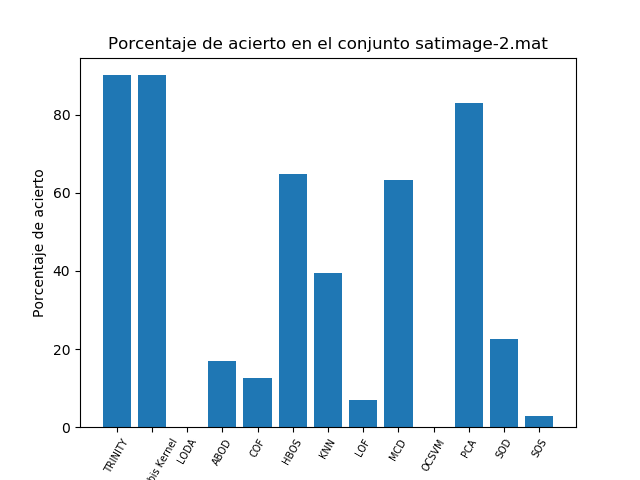
\includegraphics[scale=0.7]{imagenes/imgs-exp1/accuracy/satimage-2}
	\caption{Porcentaje de acierto sobre el conjunto de datos satimage-2}
\end{figure}

\begin{figure}[H]
	\centering
	\label{speech_accuracy}
	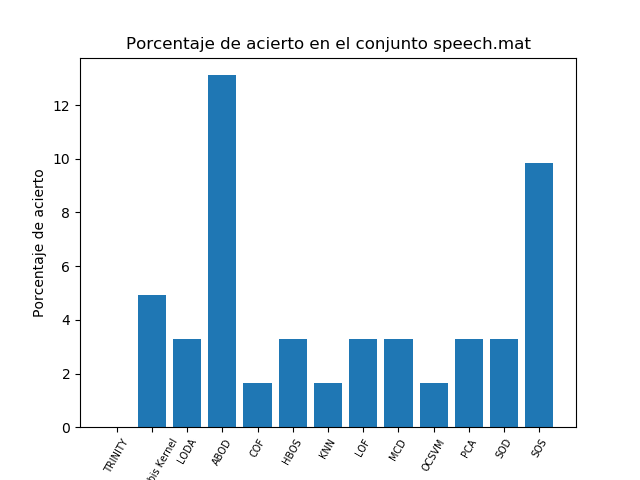
\includegraphics[scale=0.7]{imagenes/imgs-exp1/accuracy/speech}
	\caption{Porcentaje de acierto sobre el conjunto de datos speech}
\end{figure}

\begin{figure}[H]
	\centering
	\label{thyroid_accuracy}
	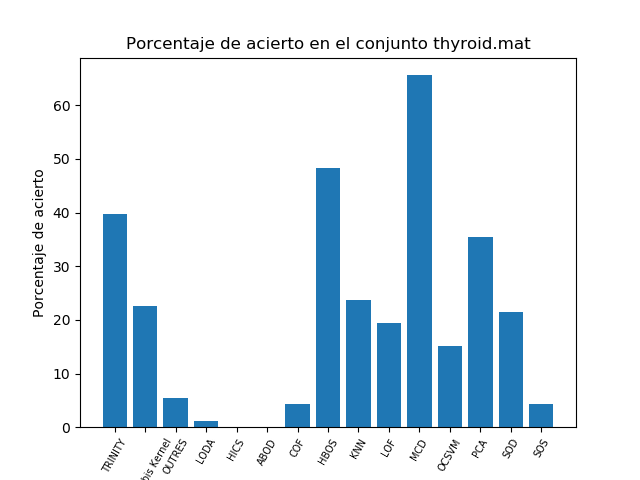
\includegraphics[scale=0.7]{imagenes/imgs-exp1/accuracy/thyroid}
	\caption{Porcentaje de acierto sobre el conjunto de datos thyroid}
\end{figure}

\begin{figure}[H]
	\centering
	\label{vertebral_accuracy}
	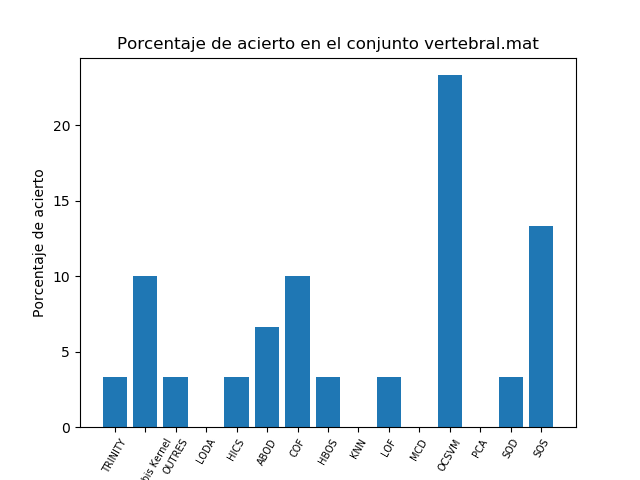
\includegraphics[scale=0.7]{imagenes/imgs-exp1/accuracy/vertebral}
	\caption{Porcentaje de acierto sobre el conjunto de datos vertebral}
\end{figure}

\begin{figure}[H]
	\centering
	\label{vowels_accuracy}
	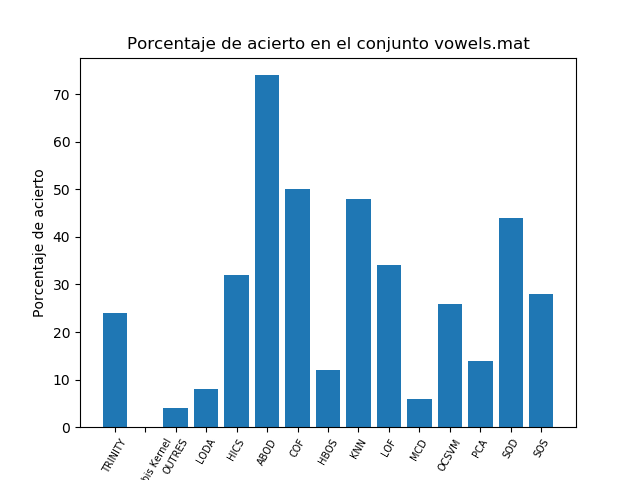
\includegraphics[scale=0.7]{imagenes/imgs-exp1/accuracy/vowels}
	\caption{Porcentaje de acierto sobre el conjunto de datos vowels}
\end{figure}

\begin{figure}[H]
	\centering
	\label{wbc_accuracy}
	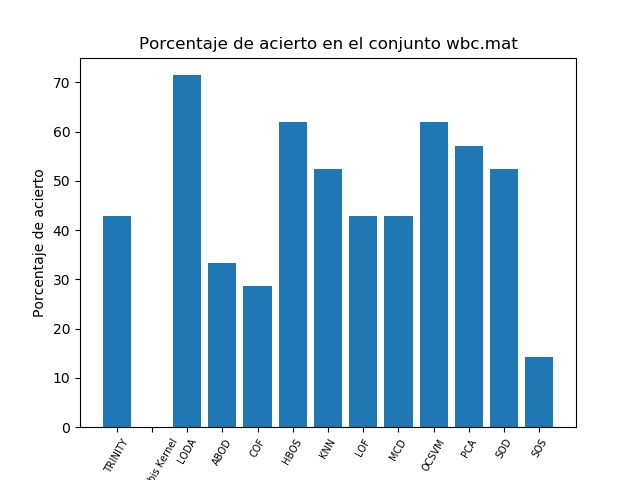
\includegraphics[scale=0.7]{imagenes/imgs-exp1/accuracy/wbc}
	\caption{Porcentaje de acierto sobre el conjunto de datos wbc}
\end{figure}

\begin{figure}[H]
	\centering
	\label{wine_accuracy}
	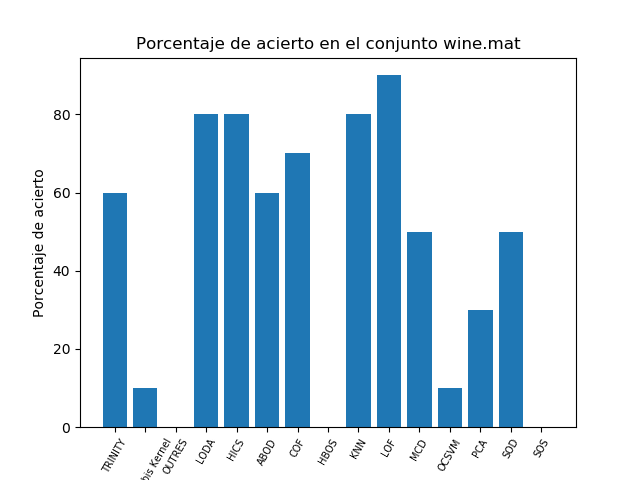
\includegraphics[scale=0.7]{imagenes/imgs-exp1/accuracy/wine}
	\caption{Porcentaje de acierto sobre el conjunto de datos wine}
\end{figure}

Como podemos observar los resultados que hemos obtenido han sido variados. En primer lugar cabe justificar algunos valores en función de la dificultad de la tarea. Como hemos comentado en la parte teórica el concepto de anomalía es algo difícil de enmarcar por lo que también es algo complejo de detectar y por tanto en función de cada conjunto de datos puede que detectemos mejor o peor sus anomalías. Por eso por ejemplo tenemos conjuntos de datos como \ref{glass_accuracy} en los que el mejor de los resultados apenas es poco más de un 20\% o \ref{optdigits_accuracy} en el que ni siquiera llegamos a dicho 20\%. Esto no es más que el reflejo de la dificultad del problema. Lo interesante de este estudio es si conseguimos mejorar en algún caso con respecto a los modelos tradicionales y la respuesta es que alguno de los modelos que hemos implementado superan en ciertos conjuntos de datos a los clásicos.

Hemos conseguido con nuestros modelos conseguir la mejor puntuación en $8$ de $22$ conjuntos de datos. Este resultado puede no parecer significativo pero debemos considerar que tenemos el doble de modelos clásicos que de modelos de ensamblaje y que ni mucho menos todos los algoritmos clásicos están al mismo nivel. Además tenemos algoritmos clásicos de todos los tipos por lo que como podemos ver en algunos conjuntos de datos no funcionan todos bien pero alguno destaca y viceversa. 

Como podemos ver en los $22$ conjuntos de datos que hemos probado los dos modelos que peores resultados nos han arrojado de loa 5 implementados son HICS y OUTRES, es decir, los dos modelos basados en subespacios que hemos implementado. Esto no quiere decir que los dos modelos sean de poca relevancia. Creo que la idea del estudio por subespacio es algo razonable y que puede arrojar buenos resultados, pero quizás no hemos utilizado para estos dos algoritmos ningún conjunto de datos conveniente. Además creo que los algoritmos de subespacios presentados son un poco rígidos en esta concepción sin querer salirse de la misma. Por ejemplo HICS obtiene sobre todo según hemos  visto anomalías que no son triviales o claramente basadas en la definición de distancias. Es por esto que, aunque lo hayamos probado como un modelo sólo, pienso que es un algoritmo más idóneo para aplicarlo en conjunción con otro tipo de algoritmos. Por ejemplo sería interesante aplicar un algoritmo basado en subespacios después de aplicar Mahalanobis Kernel puesto que este modelo y Trinity son los más fiables de los 5 que hemos estudiado. Por ejemplo podemos ver que en \ref{arrhythmia_accuracy}, \ref{breastw_accuracy}, \ref{mnist_accuracy} o \ref{satimage-2_accuracy} tanto Trinity como Mahalanobis Kernel funcionan muy bien. 

Hay un dato bastante interesante en la comparativa entre Mahalanobis Kernel y Trinity. Como hemos visto en la explicación de los modelos Trinity tiene a Mahalanobis Kernel en el primer componente. Esto en los resultados se refleja en que Trinity en general obtiene mejores resultados que Mahalanobis Kernel. El segundo componente vimos que era KNN, comparando con este modelo vemos que los resultados que obtiene Trinity son al menos iguales aunque en varios conjuntos son mejores los de Trinity que los de KNN. Por último el tercer componente de Trinity es IForest que no ha entrado dentro de esta comparativa por ser un modelo de ensamblaje también y por tanto carece de sentido contraponerlo con nuestros modelos. Esto nos está mostrando que efectivamente la combinación de modelos hace que los resultados sean más robustos obteniendo mejores resultados en general o en el peor caso manteniendo aproximadamente los resultados del modelo individual.

Por último podemos ver que LODA en general no tiene unos resultados muy espectaculares. Aún así consigue ponerse en cabeza en \ref{breastw_accuracy}, \ref{cardio_accuracy}, \ref{mammography_accuracy}, \ref{pima_accuracy} y \ref{wbc_accuracy}. En el resto de conjuntos de datos no obtiene unos buenos resultados, lo que nos está diciendo que funciona muy bien en conjuntos de datos adecuados.

Vamos a ver ambos conjuntos de datos para comprobar la razón de este comportamiento.

\begin{figure}[H]
	\centering
	\label{breastw}
	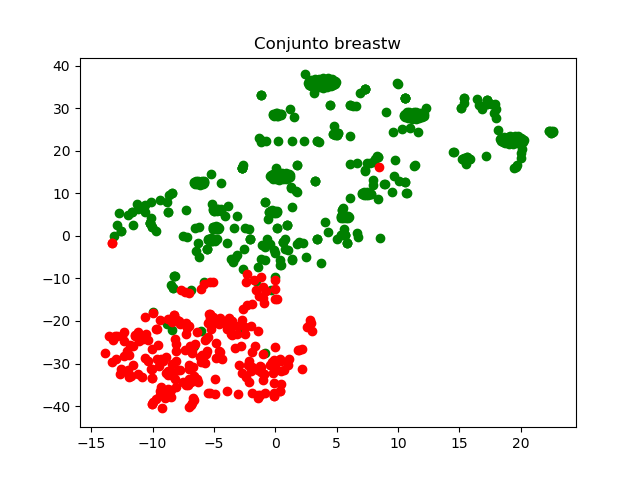
\includegraphics[scale=0.7]{imagenes/breastw}
	\caption{Proyección de breastw}
\end{figure}

\begin{figure}[H]
	\centering
	\label{glass}
	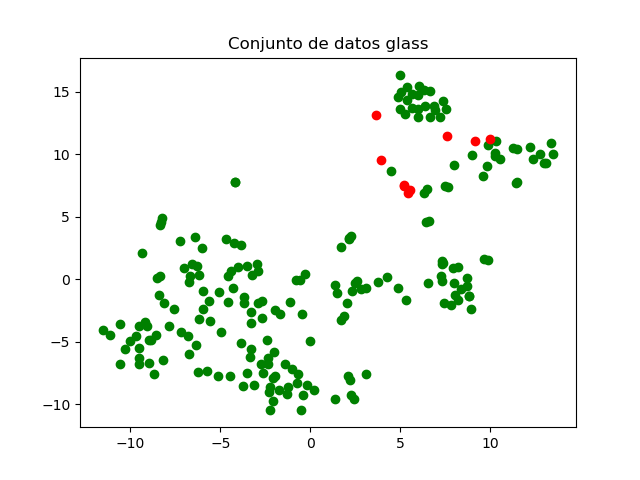
\includegraphics[scale=0.7]{imagenes/glass}
	\caption{Proyección de glass}
\end{figure}

Como podemos ver en las figuras primeras LODA funciona muy bien sobre el conjunto de datos breastw y muy mal sobre el conjunto de datos glass. Para comprobar la forma de estos dos conjuntos de datos hemos dibujado la proyección en dos dimensiones utilizando la técnica TSNE. Como podemos observar en el conjunto de datos breastw tenemos las anomalías muy separadas del resto de los datos (siendo las anomalías los datos en rojo) mientras que en glass están dentro de los datos que consideraríamos normales. Esto nos está diciendo que cuanto mayor sea la aparición de anomalías del tipo basadas en distancias mejor es el desempeño de LODA. 

Como podemos ver casi todos los modelos fallan en conjuntos de datos como optdigits. Veamos su proyección para intentar entenderlo.

\begin{figure}[H]
	\centering
	\label{optdigits}
	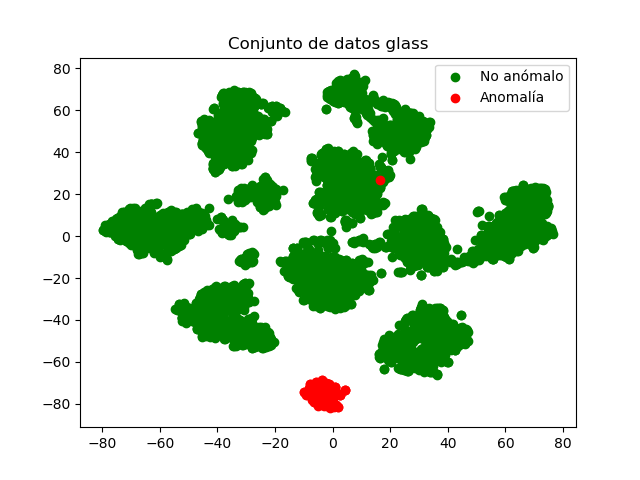
\includegraphics[scale=0.7]{imagenes/optdigits}
	\caption{Proyección de optdigits}
\end{figure}

Podría parecer que el mal desempeño de los algoritmos sea completamente ilógico al ver que las anomalías están completamente diferenciadas de los datos. Como podemos ver no sólo están separadas del resto de los datos, si no que además están muy apiñadas entre sí. Esto es un inconveniente tremendo en la detección de anomalías. Como vimos en la primera de las definiciones las anomalías deben ser datos cuya distancia al centroide sea alta cosa que no pasa en este conjuntos de datos. Si nos fijamos en la segunda definición estamos intentando estudiar la densidad de datos para ver la anomalía pero este cluster tiene una alta densidad con lo que los datos no entrarían en la definición. Este conjunto de datos refleja perfectamente la complejidad del problema. Tenemos empíricamente determinadas las anomalías pero no entran claramente en las definiciones que podemos proveer de las mismas con lo que nos es difícil clasificarlas.

HICS tiene un desempeño razonablemente bueno en el conjunto de datos wine con lo que vamos a ver su proyección e intentar sacar conclusiones.

\begin{figure}[H]
	\centering
	\label{wine}
	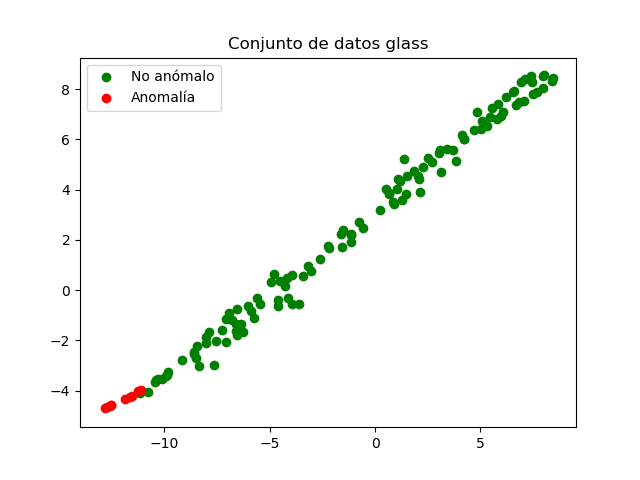
\includegraphics[scale=0.7]{imagenes/wine}
	\caption{Proyección de wine}
\end{figure}

La proyección nos está mostrando que los datos están esparcidos a lo largo de un eje con lo que podemos explicar perfectamente también el buen desempeño de Mahalanobis Kernel. En concreto podemos deducir que HICS entiende que estos datos son anómalos o al menos más anómalos que el resto de los datos porque tienen una menor densidad en su entorno. Claramente es el punto en el que menos datos hay alrededor por lo que podemos ver razonable el comportamiento satisfactorio de HICS.

Para comprender el comportamiento de outres es buena idea comprobar no sólo cuándo tenemos buenos resultados, si no que además por el propio algoritmo podemos ver el subespacio de los datos en el que cada dato es anómalo.

OUTRES no obtiene demasiados resultados satisfactorios pero donde mejor funciona es en breastw y en pima. Ya hemos visto cómo es la proyección de breastw, veamos la de pima.

\begin{figure}[H]
	\centering
	\label{pima}
	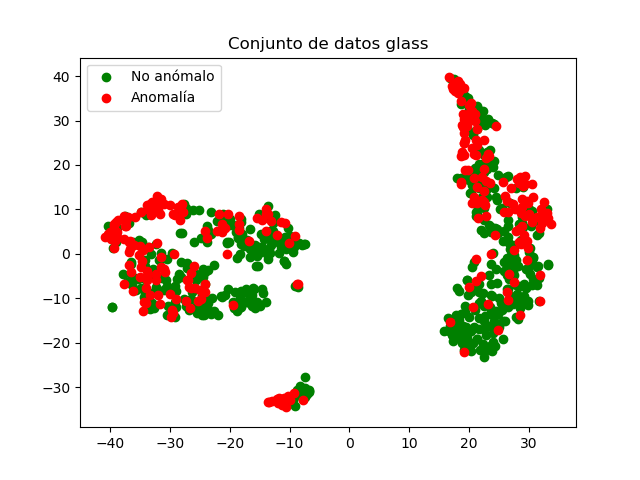
\includegraphics[scale=0.7]{imagenes/pima}
	\caption{Proyección de pima}
\end{figure}

En un primer vistazo este conjunto de datos parece bastante complejo para obtener buenos resultados, por lo que merece la pena que veamos algunos de los subespacios en los que las instancias son anómalas para así poder entender un poco mejor el resultado. Estas imágenes son de todos los subespacios posibles obtenidos por outres para cada instancia (en rojo) junto con el vecindario (en azul). Si tiene dimensión 2 se pintan directamente, si tienen una dimensionalidad mayor se hace primero la reducción de dimensionalidad mediante la técnica TSNE. Veamos algunos ejemplos:

\begin{figure}[H]
	\centering
	\label{22}
	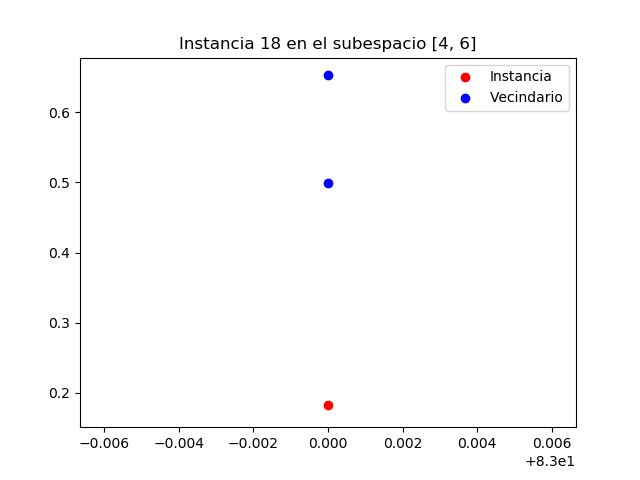
\includegraphics[scale=0.7]{imagenes/22}
	\caption{Instancia 18 sobre el subespacio $[4,6]$}
\end{figure}

Como podemos ver en dos dimensiones se comprueba rápidamente que la instancia es anómala, pero estos subespacios no son los más interesantes. Cuanto mayor es el vecindario y mayor es la dimensionalidad más conclusiones podemos obtener. Veamos uno de estos ejemplos de mayor dimensionalidad.

\begin{figure}[H]
	\centering
	\label{68_tsne}
	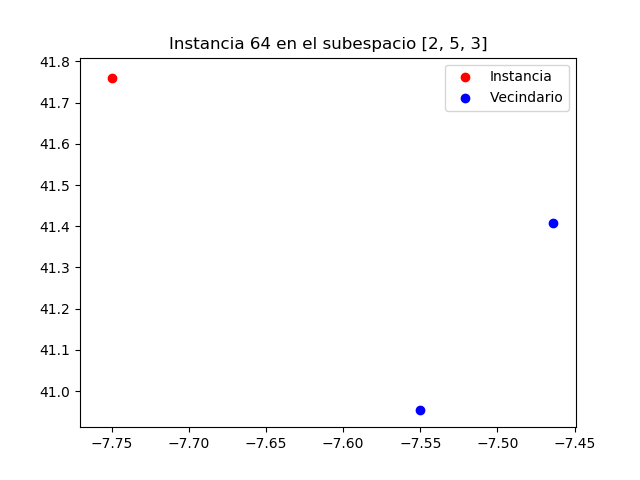
\includegraphics[scale=0.7]{imagenes/68_tsne}
	\caption{Instancia 64 sobre el subespacio $[2,5,3]$}
\end{figure}

Como podemos ver en este caso tenemos un subespacio de dimensión 3. Las instancias azules están más próximas entre sí que con respecto a la roja por lo que es normal que esta sea considerada anómala en este subespacio pues está aislada.

\begin{figure}[H]
	\centering
	\label{173_tsne}
	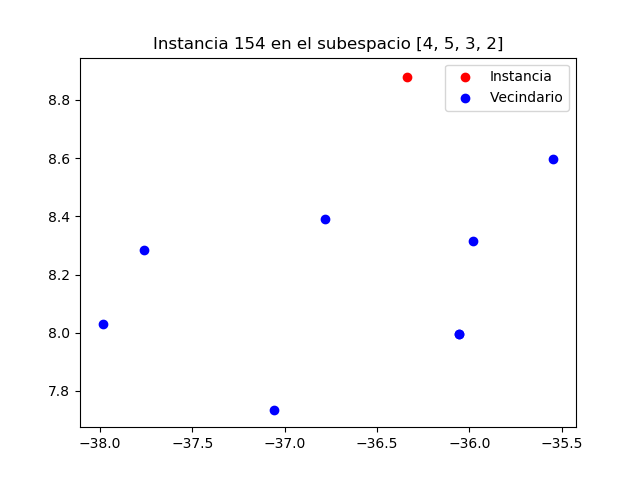
\includegraphics[scale=0.7]{imagenes/173_tsne}
	\caption{Instancia 154 sobre el subespacio $[4,5,3,2]$}
\end{figure}

Este ejemplo es de un subespacio de dimensionalidad 4. Aquí podemos ver claramente que de nuevo la instancia no sólo se encuentra algo aislada, si no que se encuentra en lo que podemos calificar como una zona poco densa con respecto a sus vecinos. Por ejemplo el dato central de esta figura no podría ser nunca considerado una anomalía en este subespacio concreto, pues al menos el vecindario sería como mínimo el que estamos observando y por tanto vemos que no es un dato raro, de hecho es el centroide de este vecindario.

\begin{figure}[H]
	\centering
	\label{190_tsne}
	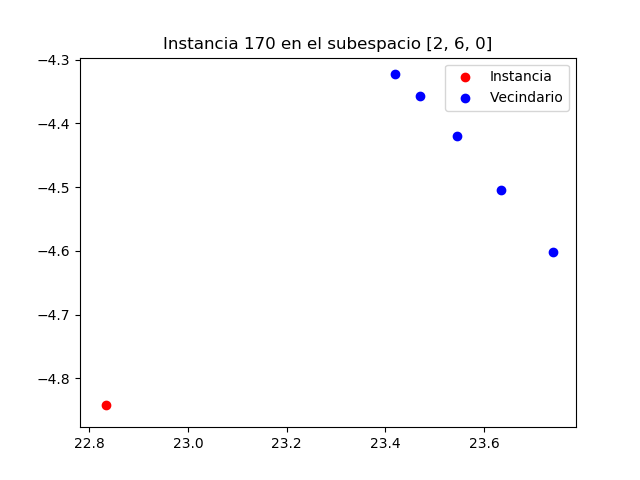
\includegraphics[scale=0.7]{imagenes/190_tsne}
	\caption{Instancia 170 sobre el subespacio $[2,6,0]$}
\end{figure}

Este ejemplo es aún más esclarecedor pues como podemos ver los datos normales están no sólo muy concentrados, si no además alineados. Esta idea de encontrar alineamiento en subespacios podría ser una buena característica a buscar en subespacios para poder emplear en ellos técnicas como Mahalanobis Kernel.

Para que sea más fácil ver los datos de acierto, vamos a ponerlos en una tabla.

% Please add the following required packages to your document preamble:
% \usepackage[normalem]{ulem}
% \useunder{\uline}{\ul}{}
\begin{table}[H]
	\resizebox{\textwidth}{!}{
	\begin{tabular}{|c|c|c|c|c|c|c|c|c|c|c|c|c|c|c|c|}
		\hline
		{\ul \textbf{Data / Mod}} & \textbf{Trinity}   & \textbf{MK}        & \textbf{OUTRES} & \textbf{LODA}      & \textbf{HICS} & \textbf{ABOD}      & \textbf{COF}       & \textbf{HBOS}      & \textbf{KNN} & \textbf{LOF}       & \textbf{MCD}       & \textbf{OCSVM}     & \textbf{PCA}       & \textbf{SOD}       & \textbf{SOS} \\ \hline
		\textbf{annthyroid}       & 26.2172\%          & 12.3595\%          & 7.4906\%        & 8.9887\%           & 6.5543\%      & 25.0936\%          & 23.0936\%          & 26.0299\%          & 28.4644\%    & 29.2134\%          & \textbf{45.8801\%} & 11.2359\%          & 23.7827\%          & 30.7116\%          & 7.4906\%     \\ \hline
		\textbf{arrhythmia}       & 48.4848\%          & \textbf{51.5151\%} & NAN             & 37.8787\%          & NAN           & 37.8787\%          & 46.9696\%          & 50\%               & 48.4848\%    & 42.4242\%          & \textbf{51.5151\%} & 15.1515\%          & 42.4242\%          & 28.7878\%          & 13.6363\%    \\ \hline
		\textbf{breastw}          & 93.3054\%          & \textbf{95.3974\%} & 50.6276\%       & \textbf{95.3974}   & 1.2552\%      & NAN                & 8.3682\%           & 93.7238\%          & 91.2133\%    & 13.3891\%          & 89.9581\%          & 91.2133\%          & 92.8870\%          & 80.7531\%          & 49.7907\%    \\ \hline
		\textbf{cardio}           & 44.3181\%          & 51.7045\%          & NAN             & 59.0909\%          & NAN           & 22.7272\%          & 19.8863\%          & 47.1590\%          & 33.5227\%    & 17.0454\%          & 40.9090\%          & 50.5681\%          & \textbf{60.7954\%} & 25.5681\%          & 10.7954\%    \\ \hline
		\textbf{glass}            & 11.1111\%          & 0\%                & 0\%             & 0\%                & 11.1111\%     & 11.1111\%          & \textbf{22.2222\%} & 0\%                & 11.1111\%    & \textbf{22.2222\%} & 0\%                & 11.1111\%          & 11.1111\%          & \textbf{22.2222\%} & 11.1111\%    \\ \hline
		\textbf{ionosphere}       & 73.0158\%          & 57.1428\%          & NAN             & 46.8253\%          & NAN           & 84.1269\%          & 77.7777\%          & 48.4126\%          & 87.3015\%    & 76.1904\%          & \textbf{88.0952\%} & 64.2857\%          & 59.5238\%          & 80.1587\%          & 61.1111\%    \\ \hline
		\textbf{letter}           & 16\%               & 15\%               & NAN             & 4\%                & NAN           & NAN                & 42\%               & 6\%                & 43\%         & 46\%               & 16\%               & 48\%               & 8\%                & \textbf{51\%}      & 6\%          \\ \hline
		\textbf{lympho}           & 83.3333\%          & 50\%               & NAN             & 0\%                & NAN           & 33.3333\%          & 50\%               & \textbf{100\%}     & 66.6666\%    & 83.3333\%          & 50\%               & 50\%               & 66.6666\%          & 50\%               & 16.6666\%    \\ \hline
		\textbf{mammography}      & 25.7692\%          & 1.1538\%           & 5.3846\%        & \textbf{28.0769\%} & 8.0769\%      & 0.3846\%           & 13.8461\%          & 12.6923\%          & 21.9230\%    & 19.2307\%          & 0.7692\%           & 27.3076\%          & 25.7692\%          & 15\%               & 5\%          \\ \hline
		\textbf{mnist}            & 40.2857\%          & \textbf{54.7142\%} & NAN             & 2\%                & NAN           & 28.5714\%          & 21.4285\%          & 17.1428\%          & 39.5714\%    & 24.2857\%          & 49.1428\%          & 0.1428\%           & 38.5714\%          & 20.5714\%          & 11.5714\%    \\ \hline
		\textbf{musk}             & 34.0206\%          & 0\%                & NAN             & 32.9896\%          & NAN           & 2.0618\%           & 8.2474\%           & 90.7216\%          & 1.0309\%     & 3.0927\%           & 96.9072\%          & 0\%                & \textbf{98.9690\%} & 4.1237\%           & 6.1855\%     \\ \hline
		\textbf{optdigits}        & 1.3333\%           & 0\%                & NAN             & 0\%                & NAN           & 4.6666\%           & 9.3333\%           & \textbf{18.6666\%} & 3.3333\%     & 10.6666\%          & 0\%                & 1.3333\%           & 0\%                & 3.3333\%           & 2.6666\%     \\ \hline
		\textbf{pendigits}        & 25\%               & 16.6666\%          & 2.5641\%        & 0\%                & NAN           & 7.0512\%           & 7.6923\%           & 32.0512\%          & 8.9743\%     & 6.4102\%           & 10.2564\%          & 26.2820\%          & \textbf{32.6923\%} & 6.4102\%           & 2.5641\%     \\ \hline
		\textbf{pima}             & 50.7462\%          & 38.8059\%          & 34.7014\%       & \textbf{54.8507\%} & 30.5970\%     & 45.8955\%          & 37.3134\%          & 50.7462\%          & 48.1343\%    & 36.9402\%          & 51.4925\%          & 39.5522\%          & 49.6268\%          & 41.4179\%          & 36.1940\%    \\ \hline
		\textbf{satellite}        & 54.3713\%          & 32.8585\%          & NAN             & 12.6227\%          & NAN           & NAN                & 43.5166\%          & 56.8271\%          & 50.0982\%    & 37.0825\%          & \textbf{68.4675\%} & 30.1571\%          & 48.3791\%          & 41.3064\%          & 29.9115\%    \\ \hline
		\textbf{satimage-2}       & \textbf{90.1408\%} & \textbf{90.1408\%} & NAN             & 0\%                & NAN           & 16.9014\%          & 12.6760\%          & 64.7887\%          & 39.4366\%    & 7.0422\%           & 63.3802\%          & 0\%                & 83.0985\%          & 22.5352\%          & 2.8169\%     \\ \hline
		\textbf{speech}           & 0\%                & 4.9180\%           & NAN             & 3.2786\%           & NAN           & \textbf{13.1147\%} & 1.6393\%           & 3.2786\%           & 1.6393\%     & 3.2786\%           & 3.2786\%           & 1.6393\%           & 3.2786\%           & 3.2786\%           & 9.8360\%     \\ \hline
		\textbf{thyroid}          & 39.7849\%          & 22.5806\%          & 5.3763\%        & 1.0752\%           & 0\%           & 0\%                & 4.3010\%           & 48.3870\%          & 23.6559\%    & 19.3548\%          & \textbf{65.5913\%} & 15.0537\%          & 35.4838\%          & 21.5053\%          & 4.3010\%     \\ \hline
		\textbf{vertebral}        & 3.3333\%           & 10\%               & 3.3333\%        & 0\%                & 3.3333\%      & 6.6666\%           & 10\%               & 3.3333\%           & 0\%          & 3.3333\%           & 0\%                & \textbf{23.3333\%} & 0\%                & 3.3333\%           & 13.3333\%    \\ \hline
		\textbf{vowels}           & 24\%               & 0\%                & 4\%             & 8\%                & 32\%          & \textbf{74\%}      & 50\%               & 12\%               & 48\%         & 34\%               & 6\%                & 26\%               & 14\%               & 44\%               & 28\%         \\ \hline
		\textbf{wbc}              & 42.8571\%          & 0\%                & NAN             & \textbf{71.4285\%} & NAN           & 33.3333\%          & 28.5714\%          & 61.9047\%          & 52.3809\%    & 42.8571\%          & 42.8571\%          & 61.9047\%          & 57.1428\%          & 52.3809\%          & 14.2857\%    \\ \hline
		\textbf{wine}             & 60\%               & 10\%               & 0\%             & 80\%               & 80\%          & 60\%               & 70\%               & 0\%                & 80\%         & \textbf{90\%}      & 50\%               & 10\%               & 30\%               & 50\%               & 0\%          \\ \hline
	\end{tabular}
}
\end{table}

Ahora para completar vamos a ver las gráficas de los tiempos consumidos por cada algoritmo para cada conjunto de datos junto con la tabla de los mismos.

\begin{figure}[H]
	\centering
	\label{annthyroid_times}
	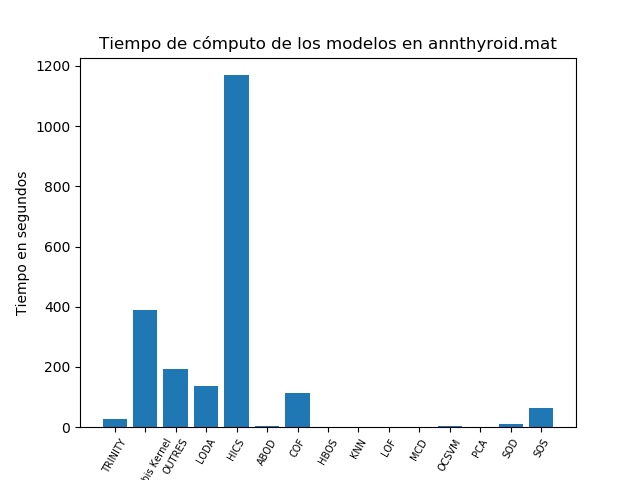
\includegraphics[scale=0.7]{imagenes/imgs-exp1/times/annthyroid}
	\caption{Tiempos sobre el conjunto de datos annthyroid}
\end{figure}

\begin{figure}[H]
	\centering
	\label{arrhythmia_times}
	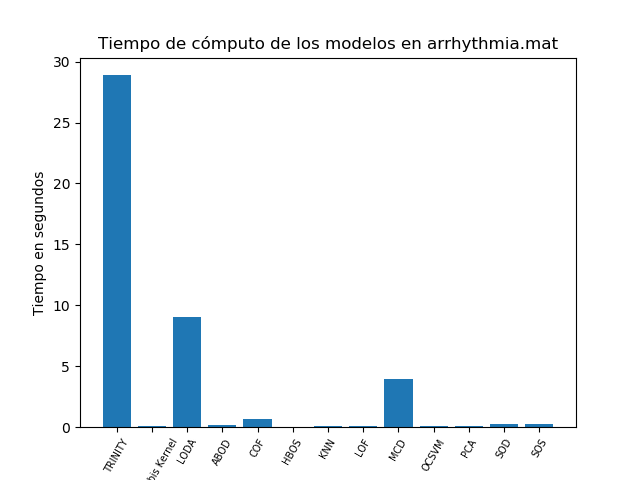
\includegraphics[scale=0.7]{imagenes/imgs-exp1/times/arrhythmia}
	\caption{Tiempos sobre el conjunto de datos arrhythmia}
\end{figure}

\begin{figure}[H]
	\centering
	\label{breastw_times}
	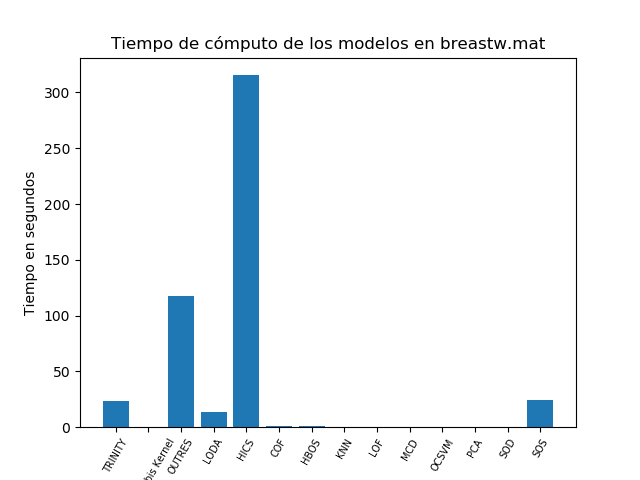
\includegraphics[scale=0.7]{imagenes/imgs-exp1/times/breastw}
	\caption{Tiempos sobre el conjunto de datos breastw}
\end{figure}

\begin{figure}[H]
	\centering
	\label{cardio_times}
	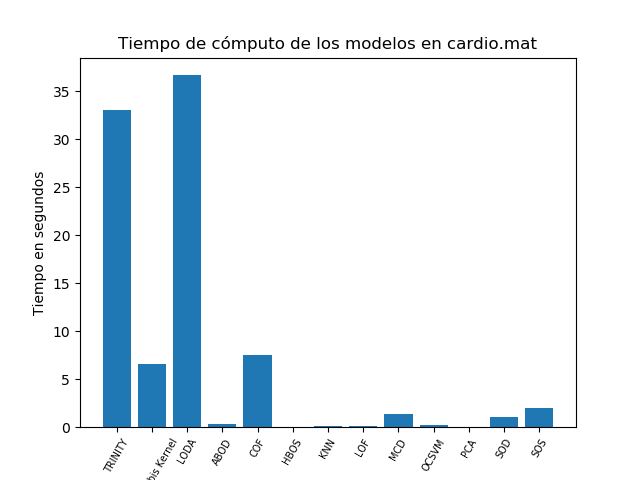
\includegraphics[scale=0.7]{imagenes/imgs-exp1/times/cardio}
	\caption{Tiempos sobre el conjunto de datos cardio}
\end{figure}

\begin{figure}[H]
	\centering
	\label{glass_times}
	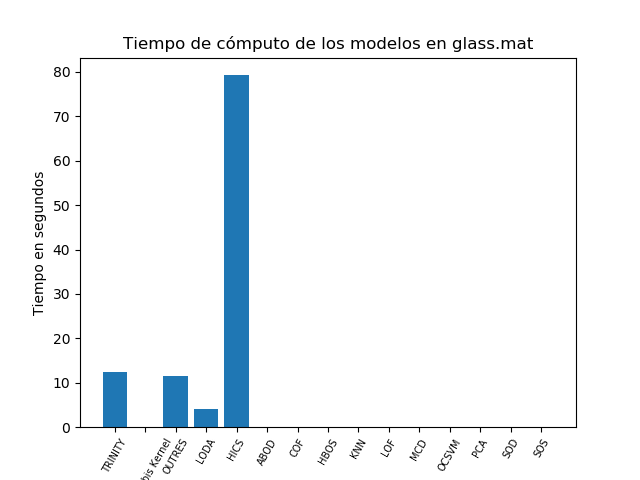
\includegraphics[scale=0.7]{imagenes/imgs-exp1/times/glass}
	\caption{Tiempos sobre el conjunto de datos glass}
\end{figure}

\begin{figure}[H]
	\centering
	\label{ionosphere_times}
	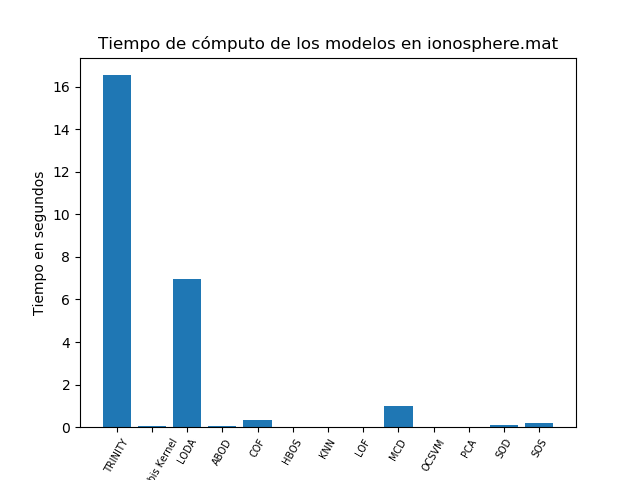
\includegraphics[scale=0.7]{imagenes/imgs-exp1/times/ionosphere}
	\caption{Tiempos sobre el conjunto de datos ionosphere}
\end{figure}

\begin{figure}[H]
	\centering
	\label{letter_times}
	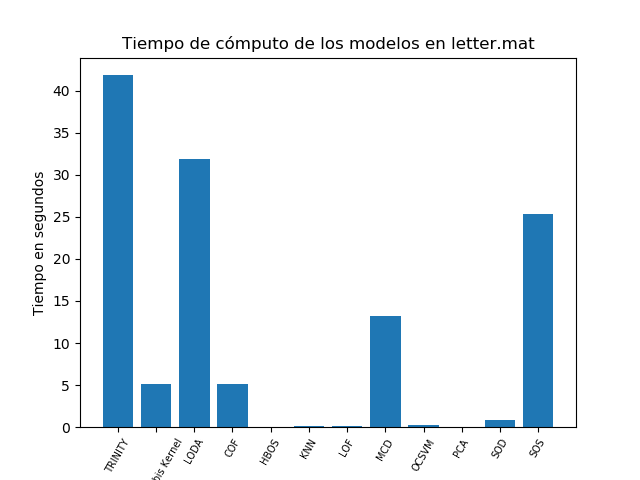
\includegraphics[scale=0.7]{imagenes/imgs-exp1/times/letter}
	\caption{Tiempos sobre el conjunto de datos letter}
\end{figure}

\begin{figure}[H]
	\centering
	\label{lympho_times}
	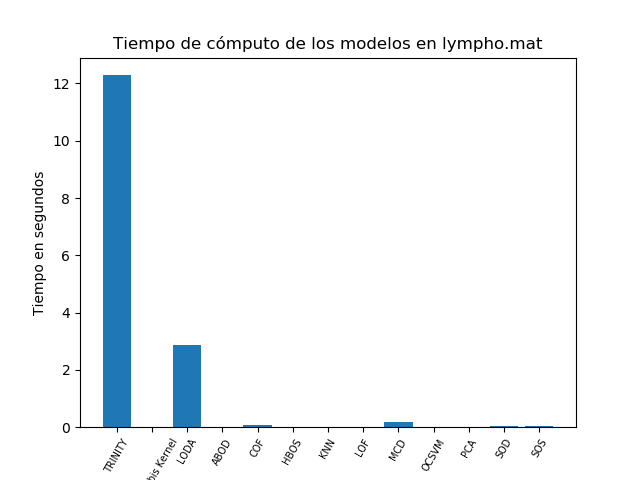
\includegraphics[scale=0.7]{imagenes/imgs-exp1/times/lympho}
	\caption{Tiempos sobre el conjunto de datos lympho}
\end{figure}

\begin{figure}[H]
	\centering
	\label{mammography_times}
	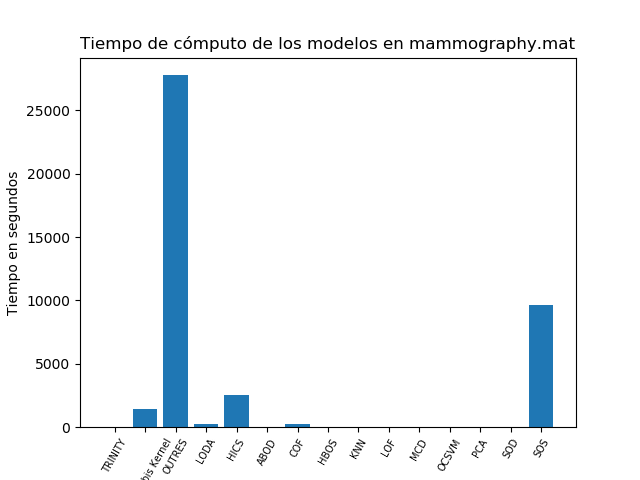
\includegraphics[scale=0.7]{imagenes/imgs-exp1/times/mammography}
	\caption{Tiempos sobre el conjunto de datos mammography}
\end{figure}

\begin{figure}[H]
	\centering
	\label{mnist_times}
	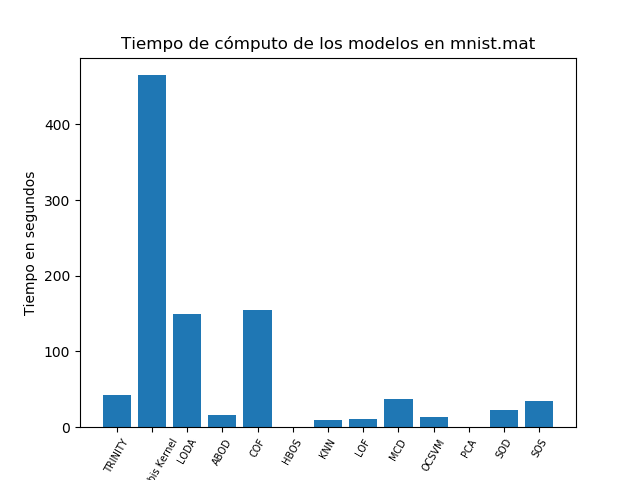
\includegraphics[scale=0.7]{imagenes/imgs-exp1/times/mnist}
	\caption{Tiempos sobre el conjunto de datos mnist}
\end{figure}

\begin{figure}[H]
	\centering
	\label{musk_times}
	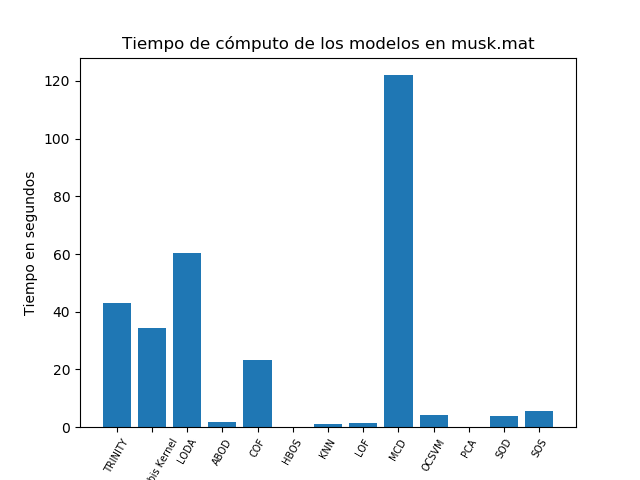
\includegraphics[scale=0.7]{imagenes/imgs-exp1/times/musk}
	\caption{Tiempos sobre el conjunto de datos musk}
\end{figure}

\begin{figure}[H]
	\centering
	\label{optdigits_times}
	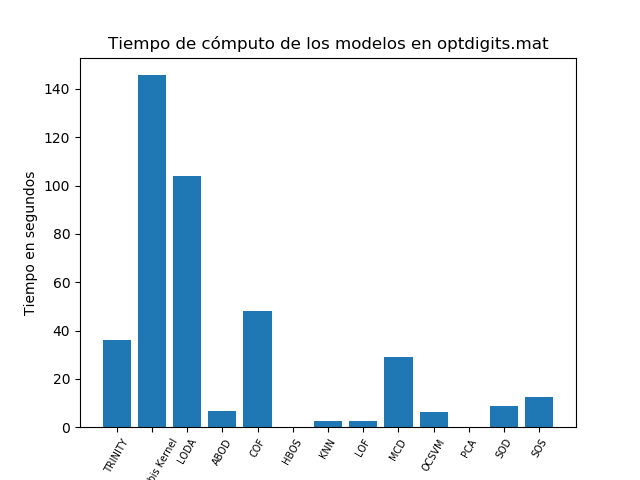
\includegraphics[scale=0.7]{imagenes/imgs-exp1/times/optdigits}
	\caption{Tiempos sobre el conjunto de datos optdigits}
\end{figure}

\begin{figure}[H]
	\centering
	\label{pendigits_times}
	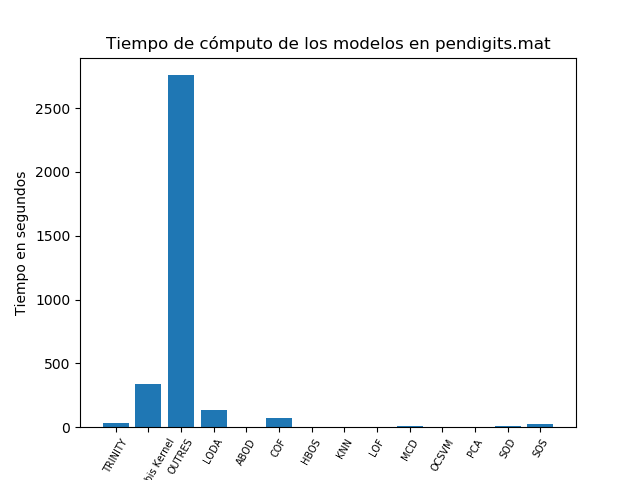
\includegraphics[scale=0.7]{imagenes/imgs-exp1/times/pendigits}
	\caption{Tiempos sobre el conjunto de datos pendigits}
\end{figure}

\begin{figure}[H]
	\centering
	\label{pima_times}
	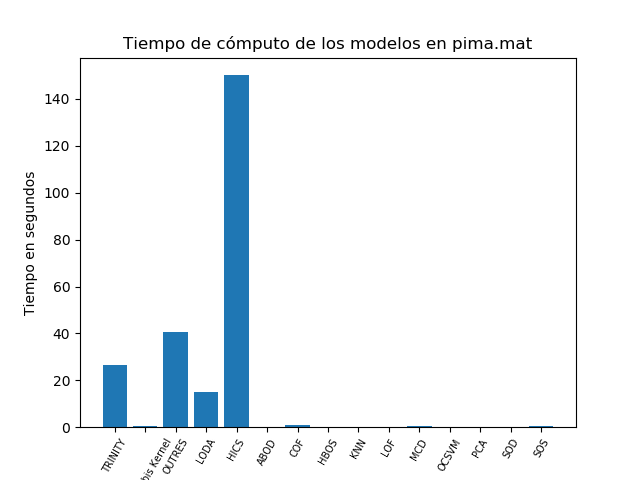
\includegraphics[scale=0.7]{imagenes/imgs-exp1/times/pima}
	\caption{Tiempos sobre el conjunto de datos pima}
\end{figure}

\begin{figure}[H]
	\centering
	\label{satellite_times}
	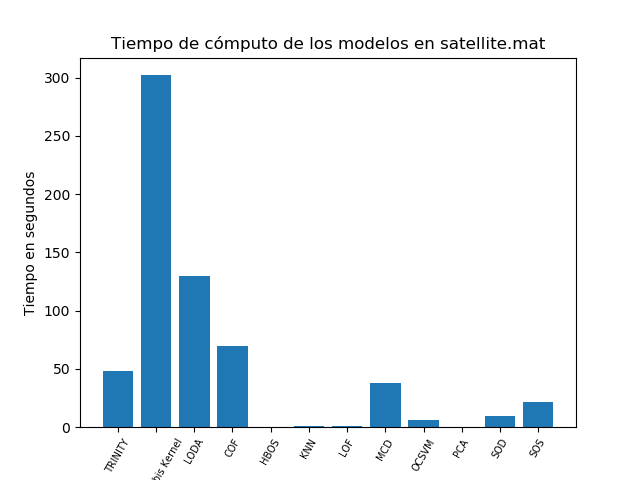
\includegraphics[scale=0.7]{imagenes/imgs-exp1/times/satellite}
	\caption{Tiempos sobre el conjunto de datos satellite}
\end{figure}

\begin{figure}[H]
	\centering
	\label{satimage-2_times}
	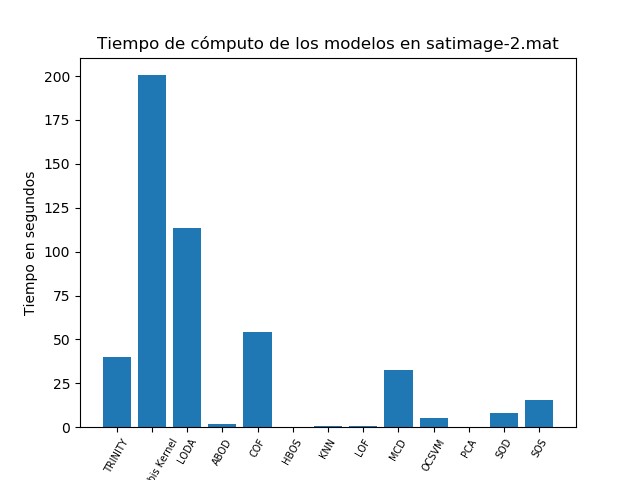
\includegraphics[scale=0.7]{imagenes/imgs-exp1/times/satimage-2}
	\caption{Tiempos sobre el conjunto de datos satimage-2}
\end{figure}

\begin{figure}[H]
	\centering
	\label{speech_times}
	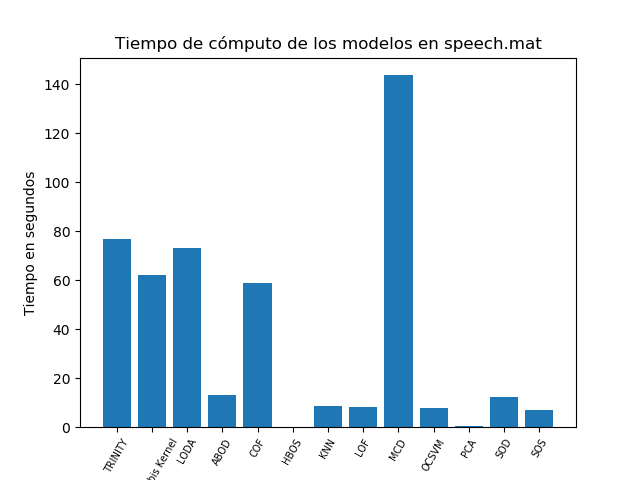
\includegraphics[scale=0.7]{imagenes/imgs-exp1/times/speech}
	\caption{Tiempos sobre el conjunto de datos speech}
\end{figure}

\begin{figure}[H]
	\centering
	\label{thyroid_times}
	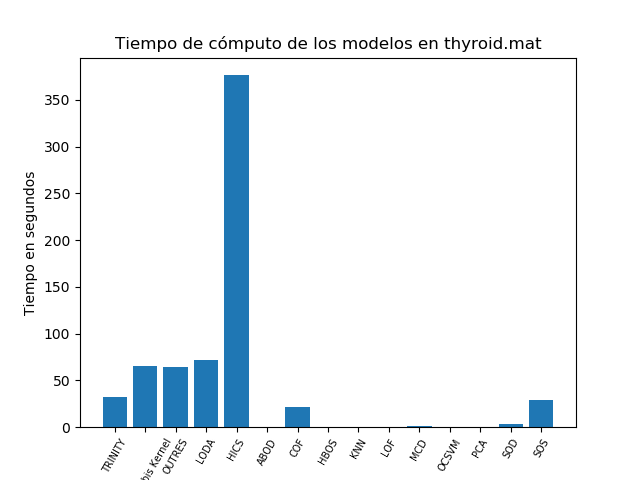
\includegraphics[scale=0.7]{imagenes/imgs-exp1/times/thyroid}
	\caption{Tiempos sobre el conjunto de datos thyroid}
\end{figure}

\begin{figure}[H]
	\centering
	\label{vertebral_times}
	\includegraphics[scale=0.7]{imagenes/imgs-exp1/times/vertebral}
	\caption{Tiempos sobre el conjunto de datos vertebral}
\end{figure}

\begin{figure}[H]
	\centering
	\label{vowels_times}
	\includegraphics[scale=0.7]{imagenes/imgs-exp1/times/vowels}
	\caption{Tiempos sobre el conjunto de datos vowels}
\end{figure}

\begin{figure}[H]
	\centering
	\label{wbc_times}
	\includegraphics[scale=0.7]{imagenes/imgs-exp1/times/wbc}
	\caption{Tiempos sobre el conjunto de datos wbc}
\end{figure}

\begin{figure}[H]
	\centering
	\label{wine_times}
	\includegraphics[scale=0.7]{imagenes/imgs-exp1/times/wine}
	\caption{Tiempos sobre el conjunto de datos wine}
\end{figure}

Hay una cosa que podemos ver claramente y es el hecho de que los algoritmos de ensamblaje consumen un tiempo mayor en general que los algoritmos clásicos. De entre los 5 algoritmos implementados que se han propuesto podemos ver que cuando OUTRES y HICS se ejecutan sobre el conjunto son los que consumen un mayor tiempo, siendo no sólo los que más tiempo consumen si no que además obtienen los mayores tiempos de todos los conjuntos de datos superando incluso los mil segundos.

Tanto Trinity como Mahalanobis Kernel y LODA tienen conjuntos de datos en los que son los algoritmos que más tardan por lo que no podemos decir que uno sea más lento que el resto. 

Veamos los tiempos en una tabla de datos.

% Please add the following required packages to your document preamble:
% \usepackage[normalem]{ulem}
% \useunder{\uline}{\ul}{}
\begin{table}[H]
\resizebox{\textwidth}{!}{
	\begin{tabular}{|c|c|c|c|c|c|c|c|c|c|c|c|c|c|c|c|}
		\hline
		{\ul \textbf{Data / Mod}} & \textbf{Trinity} & \textbf{MK}   & \textbf{OUTRES} & \textbf{LODA} & \textbf{HICS} & \textbf{ABOD} & \textbf{COF} & \textbf{HBOS} & \textbf{KNN} & \textbf{LOF} & \textbf{MCD} & \textbf{OCSVM} & \textbf{PCA} & \textbf{SOD} & \textbf{SOS}  \\ \hline
		\textbf{annthyroid}       & 28.5212 seg      & 390.5937 seg  & 193.6110 seg    & 137.8692 seg  & 1169.3422 seg & 2.5419 seg    & 114.7065 seg & 1.2222 seg    & 0.2307 seg   & 0.1145 seg   & 1.5861 seg   & 2.6132 seg     & 0.0038 seg   & 10.9631 seg  & 63.2884 seg   \\ \hline
		\textbf{arrhythmia}       & 28.8828 seg      & 0.1243 seg    & NAN             & 9.0474 seg    & NAN           & 0.1662 seg    & 0.6819 seg   & 0.0508 seg    & 0.0759 seg   & 0.0917 seg   & 3.9257 seg   & 0.1281 seg     & 0.0843 seg   & 0.2299 seg   & 0.2713 seg    \\ \hline
		\textbf{breastw}          & 23.3296 seg      & 0.3165 seg    & 117.8225 seg    & 13.2879 seg   & 315.4130 seg  & NAN           & 1.0530 seg   & 0.7055 seg    & 0.0057 seg   & 0.0098 seg   & 0.5311 seg   & 0.0200 seg     & 0.0189 seg   & 0.2007 seg   & 23.9622 seg   \\ \hline
		\textbf{cardio}           & 33.0496 seg      & 6.5851 seg    & NAN             & 36.6768 seg   & NAN           & 0.3701 seg    & 7.4887 seg   & 0.0053 seg    & 0.0872 seg   & 0.1170 seg   & 1.3748 seg   & 0.2028 seg     & 0.0051 seg   & 1.0434 seg   & 2.0196 seg    \\ \hline
		\textbf{glass}            & 12.5272 seg      & 0.0220 seg    & 11.5349 seg     & 4.0798 seg    & 79.2560 seg   & 0.0358 seg    & 0.1341 seg   & 0.0036 seg    & 0.0014 seg   & 0.0021 seg   & 0.0905 seg   & 0.0028 seg     & 0.0021 seg   & 0.0421 seg   & 0.1425 seg    \\ \hline
		\textbf{ionosphere}       & 16.5319 seg      & 0.0565 seg    & NAN             & 6.9664 seg    & NAN           & 0.0641 seg    & 0.3415 seg   & 0.0062 seg    & 0.0071 seg   & 0.0101 seg   & 0.9893 seg   & 0.0103 seg     & 0.0044 seg   & 0.0897 seg   & 0.2140 seg    \\ \hline
		\textbf{letter}           & 41.8301 seg      & 5.1648 seg    & NAN             & 31.8875 seg   & NAN           & NAN           & 5.1220 seg   & 0.0075 seg    & 0.0839 seg   & 0.1047 seg   & 13.1818 seg  & 0.2577 seg     & 0.0073 seg   & 0.8809 seg   & 25.3305 seg   \\ \hline
		\textbf{lympho}           & 12.2874 seg      & 0.0187 seg    & NAN             & 2.8804 seg    & NAN           & 0.0228 seg    & 0.0693 seg   & 0.0038 seg    & 0.0014 seg   & 0.0017 seg   & 0.1741 seg   & 0.0020 seg     & 0.0029 seg   & 0.0288 seg   & 0.0526 seg    \\ \hline
		\textbf{mammography}      & 31.5619 seg      & 1444.1323 seg & 27765.1978 seg  & 224.8207 seg  & 2502.0258 seg & 1.7394 seg    & 280.7073 seg & 0.0037 seg    & 0.2790 seg   & 0.3027 seg   & 2.3683 seg   & 5.8535 seg     & 0.0066 seg   & 25.2311 seg  & 9653.7372 seg \\ \hline
		\textbf{mnist}            & 42.7623 seg      & 464.8962 seg  & NAN             & 150.1434 seg  & NAN           & 16.4729 seg   & 154.4384 seg & 0.0502 seg    & 9.7564 seg   & 10.2119 seg  & 37.5253 seg  & 14.0057 seg    & 0.1746 seg   & 22.8423 seg  & 34.5968 seg   \\ \hline
		\textbf{musk}             & 42.8683 seg      & 34.4336 seg   & NAN             & 60.4207 seg   & NAN           & 1.6461 seg    & 23.2048 seg  & 0.0555 seg    & 1.1578 seg   & 1.3294 seg   & 121.9505 seg & 4.1720 seg     & 0.2416 seg   & 3.8690 seg   & 5.7815 seg    \\ \hline
		\textbf{optdigits}        & 36.2723 seg      & 145.6876 seg  & NAN             & 103.9115 seg  & NAN           & 6.6622 seg    & 47.9141 seg  & 0.0312 seg    & 2.3891 seg   & 2.4586 seg   & 29.2400 seg  & 6.0881 seg     & 0.0513 seg   & 8.8440 seg   & 12.5010 seg   \\ \hline
		\textbf{pendigits}        & 34.0999 seg      & 340.2855 seg  & 2757.0345 seg   & 135.0839 seg  & NAN           & 1.4151 seg    & 75.1194 seg  & 0.0076 seg    & 0.3140 seg   & 0.4336 seg   & 6.3704 seg   & 3.1717 seg     & 0.0105 seg   & 10.5999 seg  & 25.3345 seg   \\ \hline
		\textbf{pima}             & 26.3576 seg      & 0.3482 seg    & 40.6379 seg     & 15.2128 seg   & 150.1283 seg  & 0.1230 seg    & 0.9667 seg   & 0.0021 seg    & 0.0053 seg   & 0.0057 seg   & 0.5652 seg   & 0.0567 seg     & 0.0028 seg   & 0.2303 seg   & 0.4855 seg    \\ \hline
		\textbf{satellite}        & 48.2618 seg      & 301.9960 seg  & NAN             & 129.6712 seg  & NAN           & NAN           & 70.0058 seg  & 0.0146 seg    & 0.7749 seg   & 0.8185 seg   & 38.1214 seg  & 6.5430 seg     & 0.0305 seg   & 9.8771 seg   & 21.9062 seg   \\ \hline
		\textbf{satimage-2}       & 39.7535 seg      & 200.5037 seg  & NAN             & 113.2818 seg  & NAN           & 1.7584 seg    & 54.0372 seg  & 0.0139 seg    & 0.7183 seg   & 0.7796 seg   & 32.5359 seg  & 5.4775 seg     & 0.0240 seg   & 8.2761 seg   & 15.4193 seg   \\ \hline
		\textbf{speech}           & 76.6633 seg      & 62.2470 seg   & NAN             & 73.0844 seg   & NAN           & 13.2967 seg   & 58.9203 seg  & 0.1523 seg    & 8.6546 seg   & 8.4023 seg   & 143.7647 seg & 7.8068 seg     & 0.5699 seg   & 12.2820 seg  & 7.1908 seg    \\ \hline
		\textbf{thyroid}          & 32.6503 seg      & 65.3469 seg   & 64.2370 seg     & 72.1607 seg   & 376.2697 seg  & 0.5982 seg    & 21.8574 seg  & 0.0022 seg    & 0.0450 seg   & 0.0676 seg   & 1.0717 seg   & 0.5607 seg     & 0.0026 seg   & 3.3138 seg   & 29.4608 seg   \\ \hline
		\textbf{vertebral}        & 13.4726 seg      & 0.0301 seg    & 1.7653 seg      & 4.6250 seg    & 9.1404 seg    & 0.0395 seg    & 0.1153 seg   & 0.0013 seg    & 0.0015 seg   & 0.0019 seg   & 0.0435 seg   & 0.0050 seg     & 0.0011 seg   & 0.0472 seg   & 0.1450 seg    \\ \hline
		\textbf{vowels}           & 36.2093 seg      & 3.1876 seg    & 426.6157 seg    & 28.2930 seg   & 5126.5627 seg & 0.2367 seg    & 3.3253 seg   & 0.0030 seg    & 0.0247 seg   & 0.0346 seg   & 0.8870 seg   & 0.0890 seg     & 0.0023 seg   & 0.6860 seg   & 1.3831 seg    \\ \hline
		\textbf{wbc}              & 17.0011 seg      & 0.0675 seg    & NAN             & 7.5109 seg    & NAN           & 0.0700 seg    & 0.2526 seg   & 0.0061 seg    & 0.0082 seg   & 0.0080 seg   & 1.7926 seg   & 0.0101 seg     & 0.0043 seg   & 0.0964 seg   & 0.2449 seg    \\ \hline
		\textbf{wine}             & 11.2756 seg      & 0.0165 seg    & 58.9642 seg     & 2.4540 seg    & 774.9212 seg  & 0.0231 seg    & 0.0421 seg   & 0.0025 seg    & 0.0010 seg   & 0.0032 seg   & 0.1075 seg   & 0.0020 seg     & 0.0020 seg   & 0.0226 seg   & 0.0539 seg    \\ \hline
	\end{tabular}
}
\end{table}

\section{Conclusiones y trabajo futuro}

Ya hemos visto todos los resultados que hemos obtenido con los modelos y el análisis de cómo funcionan de forma teórica por lo que hemos reunido todos los ingredientes necesarios para sacar algunas conclusiones sobre este estudio.

En primer lugar cabe decir que en general los algoritmos que hemos implementado (salvo los basados en subespacios) están al mismo nivel de rendimiento que los modelos clásicos. En este estudio he comprendido el potencial que podría tener un buen modelo que combine de forma adecuada modelos clásicos o incluso modelos de ensamblaje.

El enfoque de los algoritmos basados en subespacios que se han implementado no parece ser algo que funcione en conjuntos de datos reales aunque los conceptos de densidad puedan resultar interesantes por ofrecer otro punto de vista. Algoritmos como HICS y OUTRES pueden ofrecer un buen aporte extra para un modelo ya implementado, es decir, utilizar estos algoritmos para detectar lo que ellos mismos llaman anomalías no triviales. Como modelos individuales ya hemos visto que no tienen un desempeño demasiado bueno además del alto consumo en tiempo que tienen y que hace que sea difícil su aplicación en conjuntos de datos más grandes. 

Un punto de vista interesante y que se debería tener en cuenta es la aplicación de modelos en función del tipo de datos que tengamos. Es decir, un algoritmo que regule su propio comportamiento primero analizando brevemente el conjunto de datos con algunos parámetros y posteriormente ejecutando los métodos que convengan. 

Hemos podido ver en los resultados que para todos los modelos existen conjuntos de datos en los que no funcionan bien, incluso algunos llegan a sacar un 0\% tanto de los clásicos como de los algoritmos de ensamblaje. Esto nos está reflejando que no es una aproximación inteligente intentar dar un algoritmo que aplique una misma técnica para todos los conjuntos de datos con los que se encuentre.

Creo que los resultados que hemos obtenido dejan margen de mejora, lo cual hace este campo interesante y desafiante para proponer nuevas ideas sobre la mesa. En primer lugar hemos visto que todos los algoritmos tienen problemas en cuanto al manejo de los valores perdidos. Es lógico que estos algoritmos no estén preparados ante vectores que no dispongan de ningún valor numérico, pero creo que sería interesante disponer de alguna técnica que nos permita trabajar con vectores que tengan algunos valores no disponibles. Podríamos pensar por ejemplo en alguna técnica que considere la proyección del conjunto de datos sobre los atributos disponibles de esa instancia con valores perdido y hacer un estudio sobre esa proyección. Como hemos discutido previamente es fácil que, tras esas instancias con valores perdidos, se escondan anomalías reales. 

Los algoritmos como HICS y OUTRES tienen ideas teóricas muy elaboradas pero no piensan en los problemas de eficiencia que llevan tras de sí, con lo que se hacen algoritmos poco prácticos para su uso. Sería de utilidad la inclusión de técnicas inherentes a los algoritmos que mejoren su eficiencia sin reducir en exceso su desempeño. Por ejemplo la aproximación de HICS al obtener los subespacios de alto contraste siempre se queda con los de mayor contraste pero a cambio debemos hacer un cómputo desmesurado de subespacios y contrastes que disminuyen terriblemente su eficiencia.

Por contra hemos visto como Trinity consigue unos resultados robustos en comparación con los modelos que emplea. Este tipo de algoritmos de ensamblaje pueden tener mejores resultados según la experiencia que he desarrollado en este trabajo. Creo que se podrían mezclar diferentes técnicas en un algoritmo como Trinity. Por ejemplo hemos visto que hay subespacios o trozos de los conjuntos de datos en los que el alineamiento de las instancias en hiperplanos u otras formas es clara y evidente. Esto nos hace pensar en la posibilidad de usar en dichas circunstancias algoritmos como Mahalanobis Kernel. 

Todo este análisis nos está dejando claro que el futuro de los algoritmos de ensamblaje es prometedor y como línea principal de trabajo futuro para mí mismo destaco la posibilidad de crear un modelo con todo lo aprendido. Empleando las técnicas de análisis de subespacios, algoritmos basados en densidad y relación entre atributos y algoritmos basados en histogramas se podría desarrollar un modelo más completo que supere en desempeño a los estudiados en este trabajo y sobre todo a los algoritmos clásicos.